\chapter*{Decisiones}
\markboth{Decisiones}{Decisiones}
\addcontentsline{toc}{section}{Decisiones}
\label{decision}

Esta búsqueda es la verdadera búsqueda completa, la búsqueda exhaustiva. Es como la fórmula general de cualquier fuerza bruta.

La idea principal es que vamos a ver si se puede encontrar una solución que cumpla algo que pida el problema. Lo especial es que esta solución será resultado de una cadena de decisiones tomadas. Es decir, se pueden tomar decisión que hagan que se cumpla algo. 


\begin{center}
	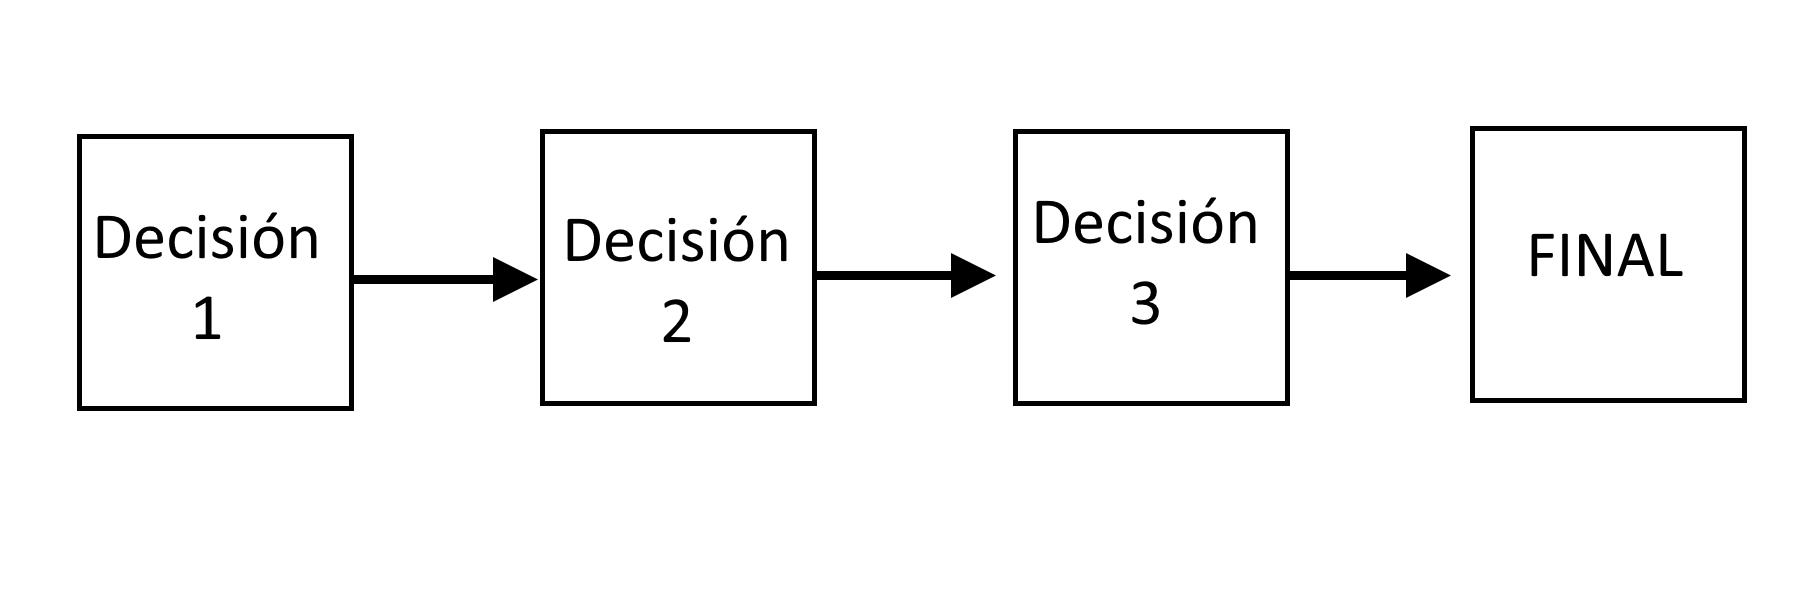
\includegraphics[scale=0.2]{decisiones}
\end{center}

Y la idea de esta búsqueda completa es revisar todas las formas posibles de tomar la serie de decisiones. 

Es decir, supongamos que estamos buscando la solución y tenemos una decisión ante nosotros con dos opciones. Lo que la búsqueda exhaustiva hace es ver "¿qué pasa si elijo la primera opción?" y luego revisa "¿Y qué sucede con la segunda opción?". Si después hay más decisiones, también explorara todas las opciones que aporten.

De forma que la búsqueda se ve aproximadamente de la siguientes dos formas:


\begin{lstlisting}
	busqueda(decision, solucion) {
		si (decision es el final) {
			revisar solucion contruida;
			return;
		}
	
		//Revisa cada opcion de esta decision:
		for (int i=0; i < decision.opciones; i++) {
			busqueda(siguiente_decision, solucion+ decision.opcion[i] );
		}
	}
\end{lstlisting}


Esta primera forma de hacer la búsqueda completa le llamamos backtracking, que significa retroceder en ingles.

Esto es porque toma una opción haciendo recursión y luego cuando hace el return o termina la función, regresa en la pila recursiva, hacer un retroceso  de su decisión.

Pero a veces conviene hacer otro tipo de búsqueda, dependiendo del tipo de decisiones a tomar, por ejemplo:

\begin{lstlisting}
	for (decision 1) {
		for (decision 2) {
			...
			for (decision n) {
				revisar solucion
			}
		}
	}
\end{lstlisting}

Esta es una idea abstracta y un poco extraña, pero es poderosa, de hecho es una forma de realizar cualquier búsqueda completa, incluyendo las búsquedas en pares, subconjuntos y ordenes.

Como siempre, ver un ejemplo ayuda mucho a entenderlo. Veamos un problema con el que ya estemos familiarizados.
\section*{Ejemplo 2.3.1}
\addcontentsline{toc}{subsection}{Ejemplo 2.3.1}
Dado un arreglo \(A\) de \(N\) enteros, determina si existe un par \(i\) y \(j\) (\(i<j\)) tal que \(A[i]+A[j]==K\).

\subsection*{Ejemplo}
\begin{casebox2}
	\scase{
		5 8\\
		3 1 2 5 9
	} 
	{SI}
	\scase{
		5 10\\
		3 4 2 12 9
	} {
		NO
	}

\end{casebox2}
\subsubsection*{Límites}
\begin{plimits}
	\item \(1\leq N \leq 10^3\)
	\item \(1\leq A[i], K \leq 10^9\)
\end{plimits}

Fuente: TODO

\section*{Solución}
Este problema lo vimos en la sección de iterar por pares, y eso es lo que debemos hacer:

\begin{lstlisting}
	bool respuesta=false;
	for (int i=0; i < N;i++) {
		for (int j=i+1; j < N; j++) {
			if (A[i]+A[j]==K) {
				respuesta=true;
			}
		}
	}
\end{lstlisting}

Pero ahora pensemos un poco a más profundidad que hace este código.

Primero va revisando todas las opciones de \(i\). Y para cada opción, evalúa todas las opciones para \(j\).

De otra forma. Podemos ver que tenemos dos decisiones, primero decidir el valor de \(i\) y luego cuanto valdrá \(j\). La primera decisión la resolvemos con el primer ciclo for y la segunda decisión con el otro for.

Visto con un código más similar al de esta búsqueda sería:

\pagebreak

\begin{lstlisting}
	int solucion[3];
	bool respuesta=false;
	void buscar(int decision) {
		if (decision==3) {
			//Ya tomamos las dos decisiones, cuanto vale i, cuanto vale j. Revisemos esta solucion
			if (A[solucion[1]]+A[solucion[2]]==K) {
				respuesta=true;
			}
			return;
		}
		if (decision == 1) {
			//toca decidir cuanto vale i. Como esto es busqueda completa, revisaremos cada opcion.
			for (int i=0;i < N; i++) {
				solucion[decision]=i;//agregar i a la solucion
				buscar(decision+1);	
				solucion[decision]=-1;//quitar i de la solucion
			}
		} else {
			//toca decidir cuanto valdra j. Probemos todos los valores
			for (int j= solucion[1]+1; j< N;j++) {				
				solucion[decision]=i;//agregar j a la solucion
				buscar(decision+1);
				solucion[decision]=i;//quitar j.
			}
		}
	}
\end{lstlisting}

Estos dos códigos siguen la misma idea de obtener los pares fijando primero un valor de i, y  luego fijando un valor para j; solo lo realizan de una forma diferente.

Entiende porque los dos códigos son iguales antes de continuar, prueba a ejecutar ambos a mano con lápiz y papel.

Básicamente el primer código hace lo siguiente para explorar todos los pares:
\begin{center}
	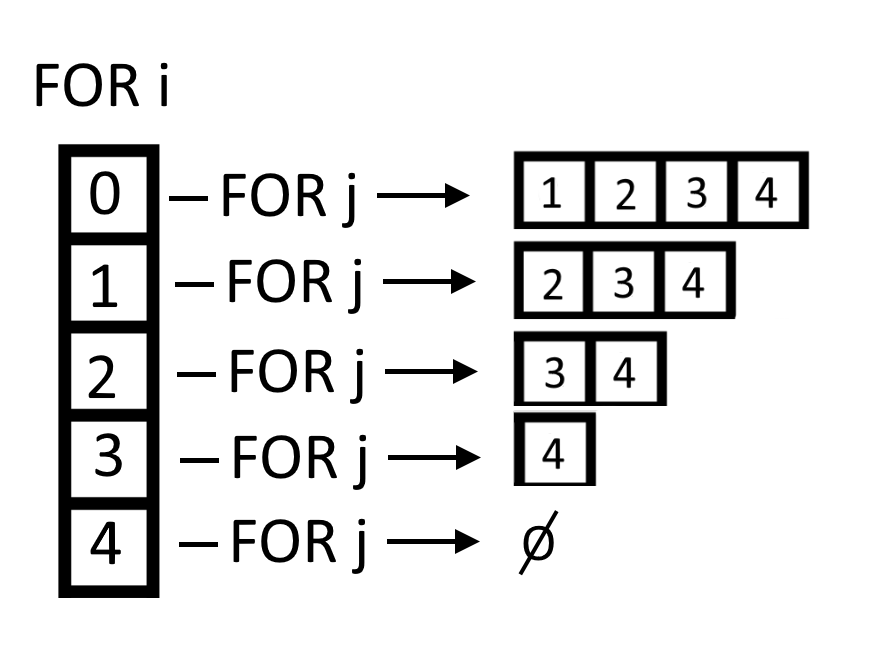
\includegraphics[scale=0.3]{forbrute}
\end{center}

Mientras que el segundo hace recursión para obtener todos los pares posibles.

\begin{center}
	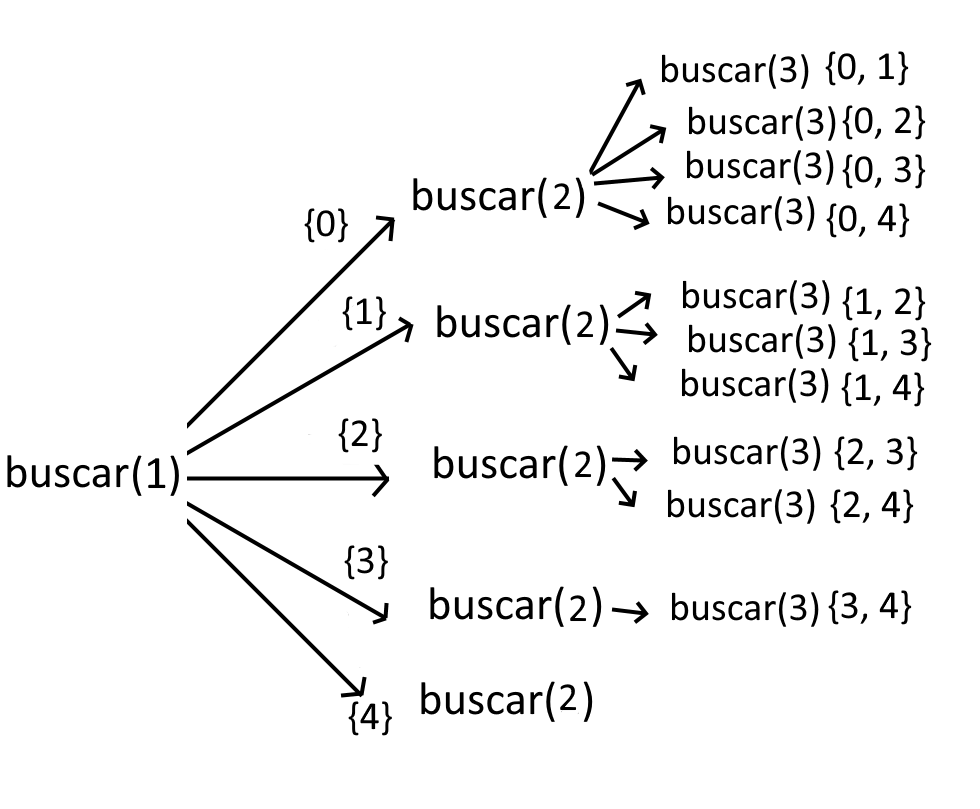
\includegraphics[scale=0.3]{paresrec}
\end{center}

Ambos son búsquedas completas que exploran todas las formas de tomar las decisiones de elegir \(i\) y luego \(j\).

\section*{Ejemplo 2.3.2}
\addcontentsline{toc}{subsection}{Ejemplo 2.3.2}

Una clase se ha juntado para jugar LaserTag. Por el diseño del lugar donde van a jugar han decidido formar tres equipos, pero quieren que los jugadores sean repartidos justamente.

La clase consiste de \(n\) estudiantes. El estudiante \(i\) tiene \(a_i\) habilidad para el LaserTag. 

Los equipos están repartidos de forma justa si la suma de la habilidad de sus integrantes es igual para los tres equipos y nadie se queda sin equipo.

Determina si se puede formar los equipos de forma justa y si sí, determina la repartición.

\subsection*{Entrada}
Un entero \(n\), indicando la cantidad de estudiantes en la clase.

La segunda línea tendrá \(n\) enteros \(a_1, a_2, \ldots, a_n\), donde \(a_i\) es la habilidad del estudiante \(i\).

\subsection*{Salida}
Si no se puede hacer la repartición imprime \verb|NO|.

En caso de que se pueda, en la primera línea imprime \verb|SI|.

En la segunda línea imprime \(n\) enteros. El \(i\)-ésimo entero sera 1, 2 o 3 dependiendo de a que equipo va el estudiante \(i\). 

Si hay varias soluciones, se acepta cualquiera.

\subsection*{Ejemplo}
\begin{casebox3}
	\ecase{
		6\\
		3 1 6 2 4 2  
	}{
	SI\\
	1 1 3 2 2 1
	}{
		El primer equipo tiene una habilidad\\ de
		\(3+1+2\).
		\\
		\\
		El segundo tiene habilidad de \(2+4\).
		\\
		\\
		Y el tercer equipo tiene un\\ integrante de \(6\).
	}
	\ecase{
		6\\
		2 1 5 2 3 4
	}{NO}{No se puede repartir a\\ los estudiantes justamente.}
\end{casebox3}

\subsection*{Límites}
\begin{plimits}
	\item \(1\leq N \leq 15\)
	\item \(1\leq a_i \leq 10^6\)
\end{plimits}

\section*{Solución}

Como siempre, antes de leer la solución te invitamos a que trates de resolver el problema por un rato.

Entonces, podemos pensarlo como que tenemos \(N\) decisiones, donde cada decisión es ¿A que equipo envío al estudiante \(i\)?

Y lo podemos imaginar como que los estudiantes se forman delante de nosotros y les vamos diciendo: "Equipo 1, equipo 2, equipo 1, equipo 3, ... ".

Entonces, podemos hacer un código que haga eso, que vaya tomando las decisiones de enviar a cada estudiante al equipo 1, 2 o 3.

Para esto crearemos la función repartir(int c, int equipo1, int equipo2, int equipo3) que se encargara de decidir a cual equipo mandar al estudiante \(c\). 
Y llevaremos cuenta de cuanta habilidad lleva cada equipo hasta ahora.

Además usaremos un arreglo \verb|reparticion[]| para llevar cuenta de a que equipo mandamos cada estudiante.

\begin{lstlisting}
int n;
int a[16];
int reparticion[16];
void repartir(int c, int equipo1, int equipo2, int equipo3) 
{
	//Mandar el estudiante c al equipo1:
	reparticion[c]=1;
	repartir(c+1, equipo1+a[c], equipo2, equipo3);
	
	//Mandar el estudiante c al equipo2:
	reparticion[c]=2;
	repartir(c+1, equipo1, equipo2+a[c], equipo3);
	
	//Mandar el estudiante c al equipo2:
	reparticion[c]=3;
	repartir(c+1, equipo1, equipo2, equipo3+a[c]);
}
\end{lstlisting}

Ahora, le falta la condición de paro. Esto será en el momento que ya no tengamos estudiantes que repartir, cuando \(c=n\).

Además, aprovecharemos allí para validar que la repartición sea justa. Si lo es, imprimiremos esta construcción como respuesta y terminaremos el programa.
\pagebreak
\begin{lstlisting}
int n;
int a[16];
int reparticion[16];
void repartir(int c, int equipo1, int equipo2, int equipo3) 
{
	if (c==n) {
		if (equipo1==equipo2 && equipo1==equipo3) {
			cout << "SI\n";
			for (int i =0;i<n; i++) 
				cout << reparticion[i]<<" ";					
			exit(0);
		}
		return;
	}
	//Mandar el estudiante c al equipo1:
	reparticion[c]=1;
	repartir(c+1, equipo1+a[c], equipo2, equipo3);
	
	//Mandar el estudiante c al equipo2:
	reparticion[c]=2;
	repartir(c+1, equipo1, equipo2+a[c], equipo3);
	
	//Mandar el estudiante c al equipo2:
	reparticion[c]=3;
	repartir(c+1, equipo1, equipo2, equipo3+a[c]);
}
int main() {
	ios_base::sync_with_stdio(0); cin.tie(0);
	cin >> n;
	for (int i =0; i< n; i++) {
		cin >> a[i];
	}
	repartir(0, 0, 0, 0);
	cout << "NO";
}

\end{lstlisting}

\section*{Complejidad}
\addcontentsline{toc}{subsection}{Complejidad}
La complejidad de una búsqueda exhaustiva varia mucho dependiendo de que tipo de solución se esta buscando, en el Ejemplo 2.3.1 vimos un ejemplo de complejidad \(O(N^2)\). 

Pero la complejidad del ejemplo anterior es \(O(3^N)\). Esto es porque la complejidad de la búsqueda exhaustiva o completa es \(O(candidatos)\) y en este caso, las formas de repartir se multiplican por tres por cada estudiante que se agregue a la clase, ya que tenemos todas las opciones de equipos anteriores, pero unas con el nuevo en el 1, otros con el equipo 2, y otra vez con el estudiante en el 3.



\practiceproblemsection{2.3}

\problemtitle Estas en una torre la cual tiene \(N\) pisos.

El piso \(i\) tendrá \(K_i\) pasadizos que le permiten ir a pisos superiores. El único piso sin pasadizos es el último, el piso \(N\).

Tu quieres ver cuantas formas hay de ir del piso \(1\) al \(N\). Dos maneras de ir del piso \(1\) al \(N\) son diferentes si en una usas un pasadizo y en la otra no.

Nota: esta prohibido tomar los pasadizos de un piso superior a uno inferior

\subsubsection*{Entrada}
Dos enteros \(N\), la cantidad de pisos en la torre.

En las siguientes \(N-1\) lineas vendrá la descripción de cada piso. 

Cada piso constará de un entero \(K_i\) representando cuantos pasadizos hay allí que conectan hacia arriba. Seguido, vendrán \(K_i\) enteros diferentes, representando a que pisos tienes un pasadizo. Solo podrás ir a pisos superiores.

\subsubsection*{Salida}
Imprime un entero que represente la cantidad de formas de ir del piso \(1\) al piso \(N\).

\subsubsection*{Ejemplo}
\begin{casebox3}
	\ecase{
		4\\
		2 2 3\\
		2 3 4\\
		1 4  
	}{3}
	{
		Tienes tres formas de llegar:\\
		\(1\rightarrow2\rightarrow3\rightarrow4\)\\
		\(1\rightarrow2\rightarrow4\)\\
		\(1\rightarrow3\rightarrow4\)\\
	}
\end{casebox3}

\subsubsection*{Límites}
\begin{plimits}
	\item \(1\leq N\leq 16\)
	\item \(1\leq K_i< N\)
\end{plimits}

\omegalink{} TODO

\problembreak

\problemtitle El COMI diseñó unos mapas futuristas. Los mapas futuristas son como los mapas de ahora, pero están impresos en una superficie transparente. Ellos tienen un archivo de varios mapas de la galaxia. Sebastian y Héctor se dieron cuenta de que existen varios mapas repetidos, por lo que desean eliminar cualquier repetición. Para esto, Sebastian toma un mapa, Héctor toma otro y ambos comparan los mapas para determinar si son iguales. Sin embargo, Héctor estaba distraído y algunos mapas se los pasaba en una posición diferente a la original. Ahora necesitan tu ayuda para comparar los dos mapas y saber si son iguales.

Un mapa está representado por una matriz cuadrada de \verb|X|s y \verb|O|s. Dos mapas son iguales si ambos tienen el mismo carácter en la misma coordenada, para todas las coordenadas.

Para validar que dos mapas son iguales, puedes aplicar cualquiera de las siguientes acciones cero o más veces sobre un mapa que quieras comparar con otro:
\begin{plimits}
	\item Rotarlo 90º.
	\item Rotarlo 180º.
	\item Rotarlo 270º.
	\item Invertirlo horizontalmente.
	\item Invertirlo verticalmente.
\end{plimits}
\begin{center}
	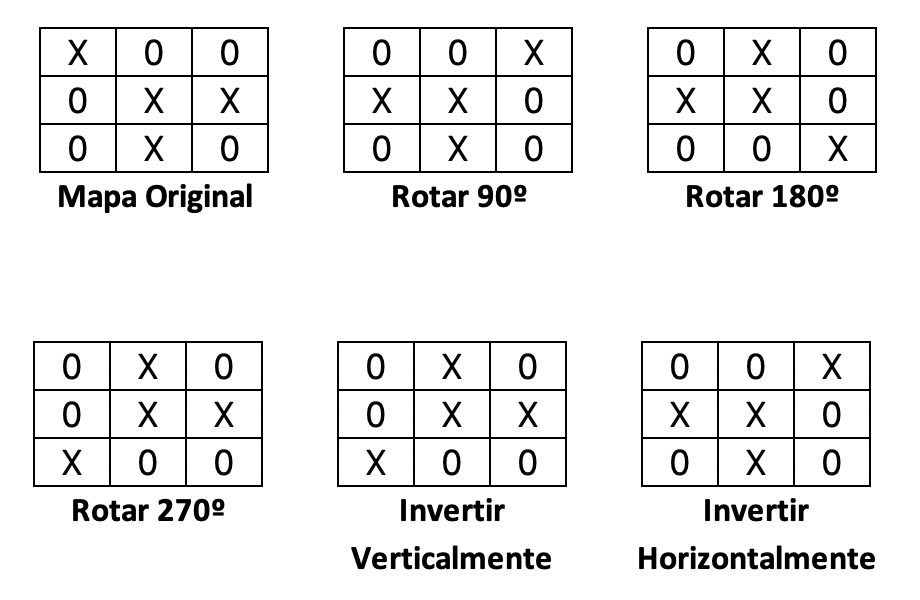
\includegraphics[scale=0.55]{mapasOMI2020}
\end{center}

\subsubsection*{Problema}
Se te mostrará dos mapas y debes ayudarles a decir si son iguales o diferentes. Si son iguales, deberás escribir \verb|IGUALES|. Si son diferentes, deberás escribir \verb|DIFERENTES|.

\subsubsection*{Entrada}
En la primera línea \(N\), la longitud del lado de cada mapa. En las siguientes \(N\) líneas una cadena de \(N\) caracteres \verb|O| ó \verb|X| que representan el primer mapa. En las siguientes \(N\) líneas una cadena de \(N\) caracteres \verb|O| ó \verb|X| que representan el segundo mapa.
\subsubsection*{Salida}
Debes escribir \verb|IGUALES| si los mapas son iguales después de hacer todas las transformaciones necesarias o \verb|DIFERENTES| en caso contrario.

\subsubsection*{Ejemplo}
\begin{casebox3}
	\ecase{
		4\\
		XOOO\\
		XXOO\\
		OOOO\\
		XXXX\\
		XOOO\\
		XOOO\\
		XOXO\\
		XOXX
	}{IGUALES}{Si el segundo mapa lo giras 90º y además\\ lo inviertes verticalmente, obtienes \\la misma distribución que el primer mapa.}
	\ecase{
		2\\
		XX\\
		OO\\
		XO\\
		OX
	}{DIFERENTES}
	{No hay manera de transformar el segundo \\mapa para que se vea tal como el primero.}
	\ecase{
		4\\
		XOOO\\
		XXOO\\
		OOOO\\
		XXXX\\
		XOOO\\
		XXOO\\
		OOOO\\
		XXXX
	}{IGUALES}{
		En este caso los mapas ya son iguales,\\ sin necesidad de aplicar ninguna operación.		
	}
\end{casebox3}

\subsubsection*{Límites}
\(1 \leq N \leq 500\)
\subsubsection*{Subtareas}
\begin{plimits}
	\item (25 puntos)
	\begin{plimits}
		\item \(1\leq N \leq 10\)
		\item Se asegura que, en caso de que los mapas sean iguales, no es necesario aplicar ninguna acción.
	\end{plimits}
	\item (25 puntos)
	\begin{plimits}
		\item \(1\leq N \leq 50\)
		\item Se asegura que, en caso de que los mapas sean iguales, no es necesario aplicar ninguna rotación.
	\end{plimits}
	\item (25 puntos)
	\begin{plimits}
		\item \(1\leq N \leq 50\)
		\item Se asegura que, en caso de que los mapas sean iguales, no es necesario aplicar ninguna inversión vertical o inversión horizontal.
	\end{plimits}
	\item (25 puntos)
	\begin{plimits}
		\item \(1\leq N \leq 500\)
		\item Cualquier acción podría ser necesaria para validar que los mapas son iguales.
	\end{plimits}
\end{plimits}
Fuente: \textbf{OMI 2020}

\omegalink{OMI-2020-Mapas}